This chapter first covers the state of the art in DT technologies in Section \ref{sec:sota}, specifically the three major aspects of monitoring, modelling, and controlling. Although these aspects do not directly address the integration and orchestration topics, however, since they are the core parts of a DT (as explained in Section \ref{sec:overview}), the DT services will certainly rely on them to achieve the intended outcomes. We reckon it is important to be informed about the state of the art in each aspect, so that when building a DT we can take this state of the art into account---including its effects on integration and orchestration.

In Section \ref{sec:relatedwork} the discussion will shift toward the available integration and orchestration approaches, and how they have been used under the context of bioprocessing DTs.

\section{State of the art}\label{sec:sota}

We review the latest developments of monitoring, modelling, and controlling respectively. Naturally, the DT services are built upon these aspects, implying the frameworks for integration and orchestration have to accommodate them in order to ensure the services running well.

\subsection{Monitoring} \label{sec:monitoring}
In DT development, the monitoring of the physical world is normally performed using sensors. Clusters of sensing nodes may work collaboratively as enabled by Internet of Things (IoT) technologies. 

\textit{Hard sensors} normally refer to the electronic instruments that detect and collect measurements directly from their vicinity, for instance, a thermostat or pressure gauge. More advanced instruments like spectroscopies---based on the interaction of electromagnetic waves and molecular bonds to measure biomass---are gaining ground \cite{Gargalo2020}. By virtue of their computing capability of properties that are obscured or out of reach to human perceptions, these sort of advanced sensors can be placed in harsh environments such as an agitated bioreactor to provide process data while maintaining non-invasive to the system. In general, high accuracy and low latency are advisable for generating reliable online data.

\textit{Soft sensors} are the inferential sensing technology that estimate process variables that cannot be directly measured, by combining data collected from hard sensors into equations and a mathematical model. Based on the techniques, they can be categorized roughly to two classes, namely \textit{model-driven} or \textit{data-driven} \cite{Udugama2021}. \textit{Model-driven} soft sensors are built upon first principles models, which rely on in-depth knowledge of the target process, and that implies higher degree of complexity. The advantage of a model-driven approach is that it has a solid foundation based on physical laws and theories, and that allows an easier generalization of the process provided the user also possesses sufficient know-how of the field \cite{Rasheed2020}. Alternatively, \textit{data-driven} sensors are fed massive data quantities in order to generate predictions. Common approaches include black-box models such as MultiVariate Data Analysis (MVDA), a form of statistical model that processes multiple variables simultaneously and eventually aims to decrease the dimensionality. Another data-driven approach that is rapidly gaining popularity is Artificial Neural Networks (ANN), thank to the wide availability of hardware support like Graphical Processing Units (GPUs), and software library support such as TensorFlow \cite{tensorflow}, and PyTorch \cite{pytorch}.

\subsection{Modelling}
Rather similar to the classifications of soft sensors described above, modeling approaches can be sorted by their level of abstraction \cite{Narayanan2020, Zhou2021}. At the higher level, techniques like first principles and mechanistic models in biochemical domains; or Computer-Aided Design (CAD) and topological models used in mechanical domains \cite{Jiang2021} are considered knowledge-based, i.e., more demanding in domain expertise, hence requiring less online data to construct. In contrast, at a lower level of abstraction, Artificial Intelligence (AI) related techniques rely more heavily on empirical data.

The step for merging the monitored data into the model states is known as data assimilation. Recursive parameter estimation is an approach for data assimilation. It refers to taking old estimates (old model parameters) obtained from fitting one set of data points to generate new estimates when new data points (new observations) are added to the original data set \cite{Rutan1990}. Another technique within the same category is extended Kalman filter, which is broadly used to perform state estimation \cite{Oisiovici2000, Kramer2016}.

Although the models used in this project are given, it is still useful to have an understanding of what modelling techniques are used these days, because different techniques consume and generate different forms of data that may require different treatments of integration and orchestration.

\subsection{Controlling}
We can consider controlling as the last piece in DTs that ``closes the loop" between the virtual world and and the physical world. Proportional–Integral–Derivative (PID) controllers have been used  in industrial control for decades. Their popularity can be attributed the robustness and simplicity in a wide range of industrial settings \cite{pidni}. On the other hand, the advancement of high volume data acquisition enables growing adoption of model predictive control (MPC), which goes beyond merely a reactive mechanism as PID, also taking into account the contextual knowledge of the underlying complex process. Hong et al. \cite{Hong2018} examine the advantage of a hybrid scheme that combines adaptive model-based feedback with direct PID control for optimizing startup, changeover, and shutdown. The study also discusses functionally partitioning components to improve flexibility and reduce operation cost for constructing hybrid models.  

In the control service which will be introduced in Chapter \ref{ch:methodology}, we use the PID approach for its simplicity as a proof-of-concept. Nonetheless, as the microbrewery DT will continue to expand and mature, we do not rule out the possibility of migrating to the MPC approach in the future. 

\section{Related work}\label{sec:relatedwork}
This section first introduces the recent progress in integration and orchestration approaches. They serve as the references for the designs to consider when choosing the frameworks in Chapter \ref{ch:methodology}. Real case studies of DT will also be described in order to show how the integration and orchestration approaches could improve DT operations.

\subsection{Integration} \label{sec:inte}
Integration is a key step of models' communication and execution. In a production plant context, communication infrastructures commonly comprise the following aspects \cite{Gargalo2020}:

\begin{itemize}

  \item A supervisory control and data acquisition (SCADA) system that handles the interfacing of monitor and control operations. Its components include remote terminal units (RTU) for processing commands; programmable logic controllers (PLC) for processing control signals; HMI for aiding the operator in various actions.
  
  \item Data standards such as XML, JSON that deliver string-value pairs of the monitoring/controlling variables. It may also contain information about the computational pipeline of the process.
  
  \item Communication protocol stacks that address each Open Systems Interconnection (OSI) layer. Common patterns such as client/server in TCP/IP, or publish–subscribe in Message Queuing Telemetry Transport (MQTT) are well documented in IoT literature.
  
\end{itemize}

It is important that the above infrastructures are classified and understood well, because in our DT construction they will become the underlying elements supporting the services to communicate information. In Chapter \ref{ch:methodology} and \ref{ch:implementation}, some of the above notions will reoccur sporadically.

Apart from the generic infrastructures, we further introduce two open source standards that target specifically the integration in modelling, namely Computer-Aided Process Engineering (CAPE)-OPEN \cite{capeopen}, and Functional Mock-up Interface (FMI) \cite{fmi, Blochwitz2011}.

\begin{figure}[hbt!]
    \centering
    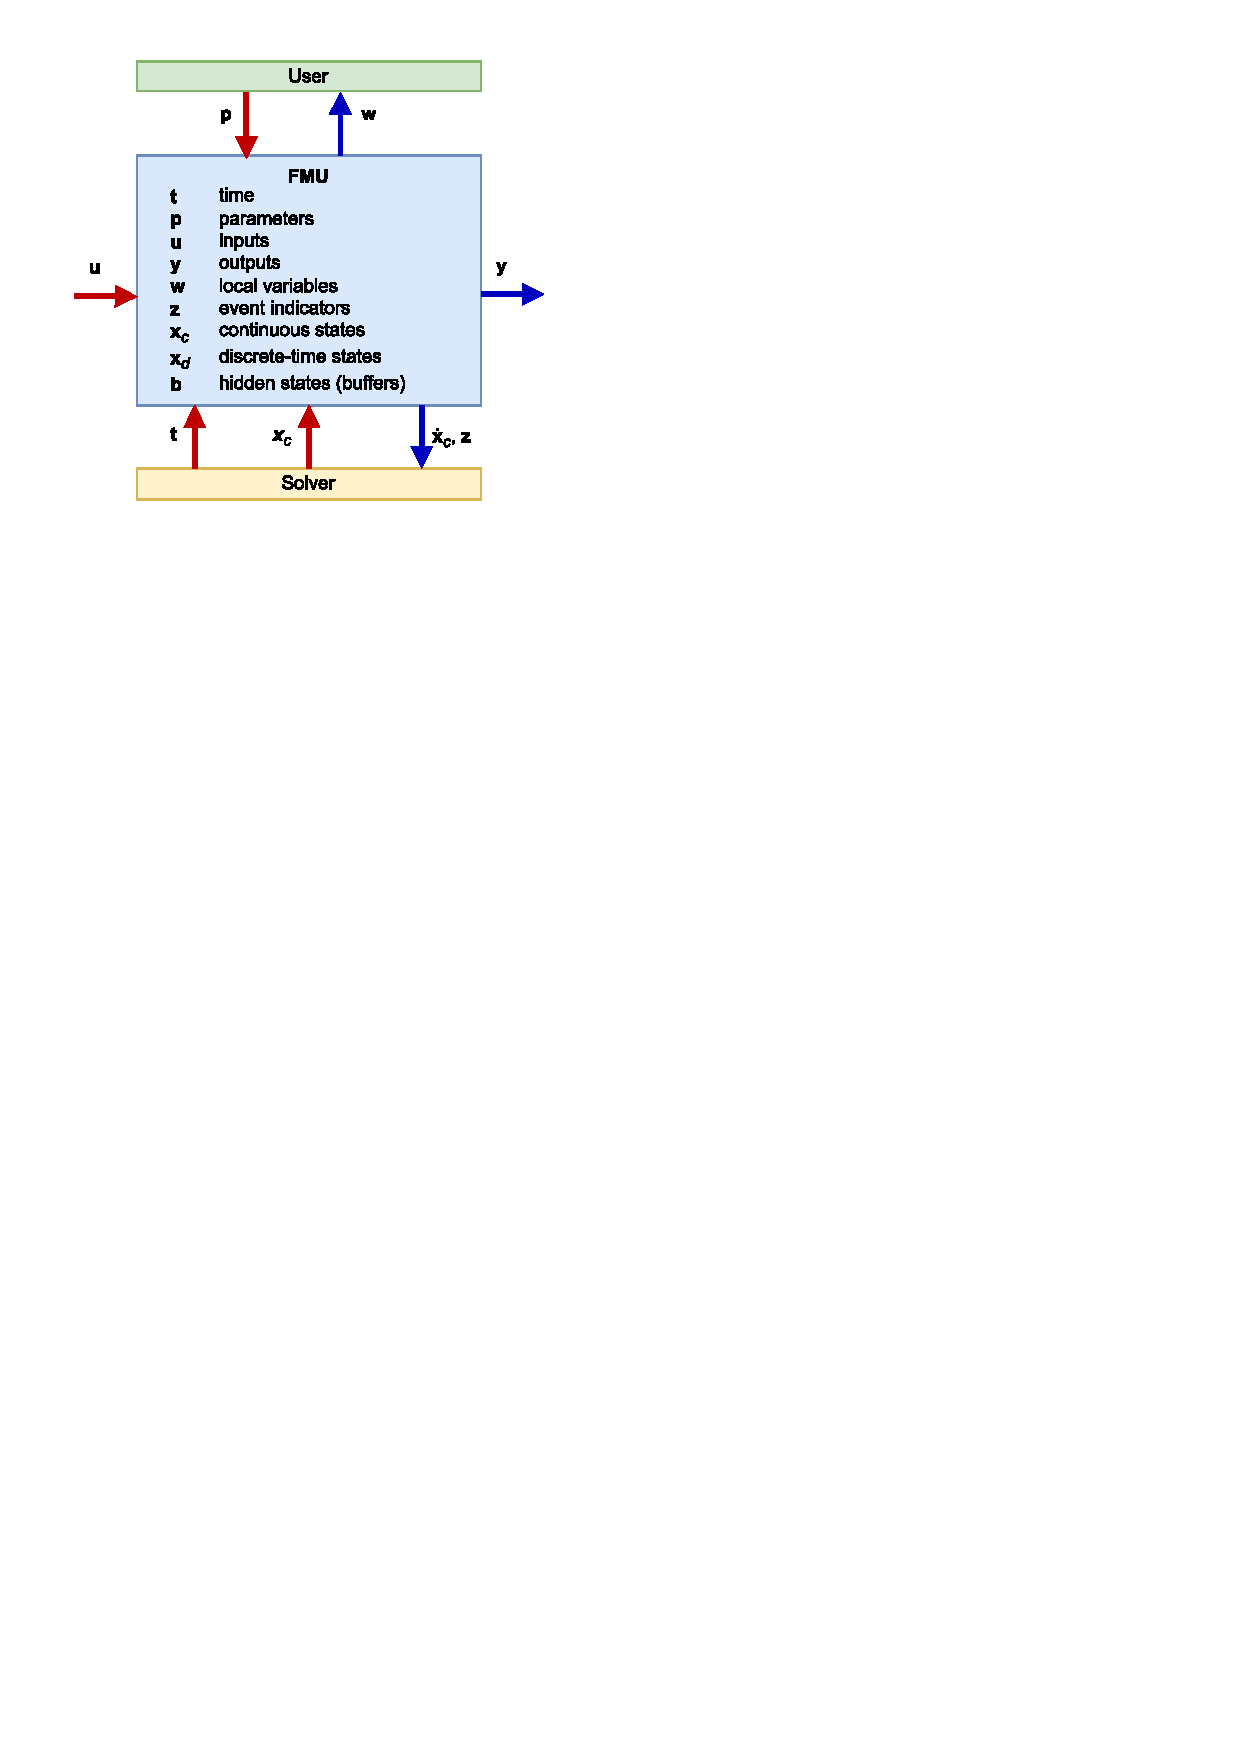
\includegraphics[scale=0.6]{figures/fmi_me.pdf}
   	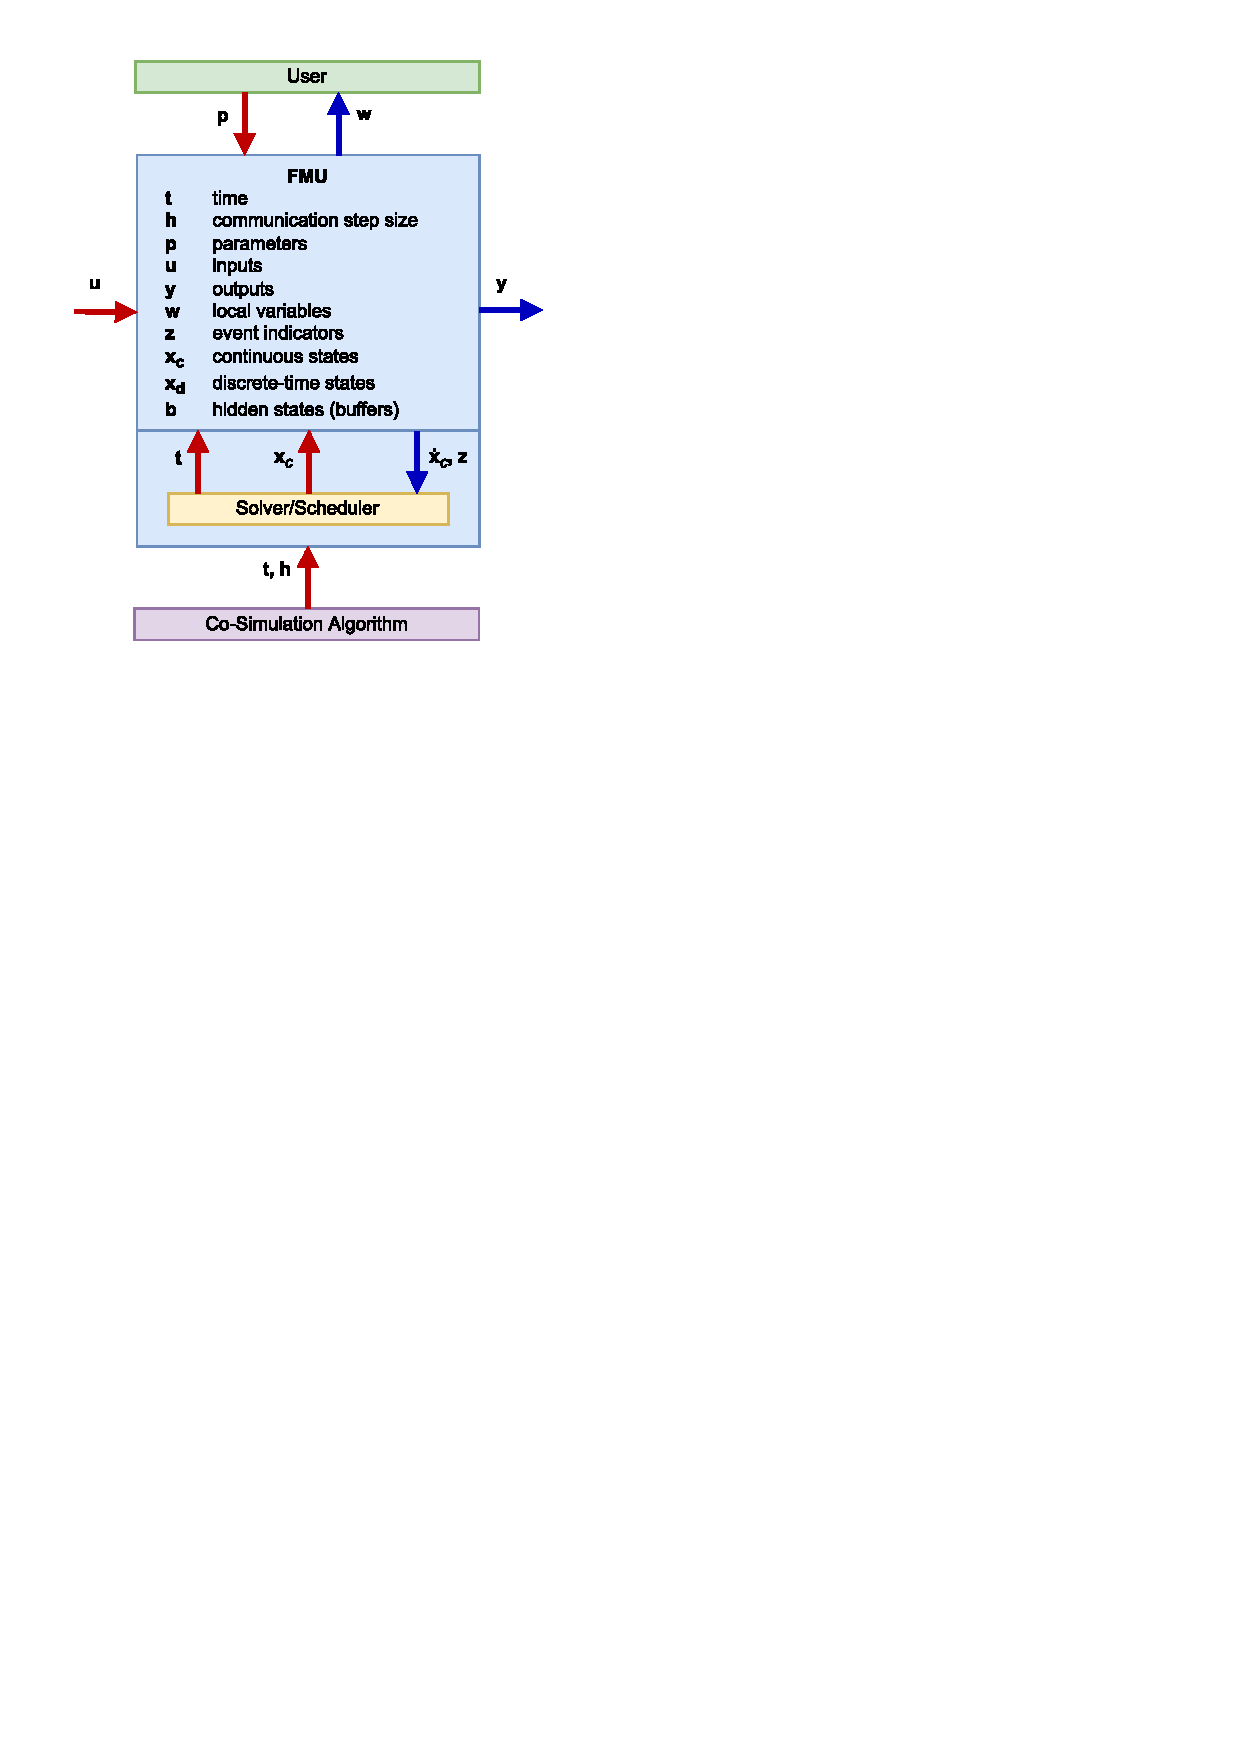
\includegraphics[scale=0.6]{figures/fmi_cs.pdf}
    \caption[FMI for model exchange (left), and FMI for co-simulation (right)] {FMI for model exchange (left), and FMI for co-simulation (right) \cite{fmidoc}}
    \label{fig:fmi}
\end{figure}

In short, CAPE-OPEN is a standard of a component-based approach to process simulation \cite{Belaud2002}, especially addressing the chemical manufacturing domain. The standard can be seen as having two parts. The first is Process Modelling Components (PMC), they represent functionally separated building blocks such as thermodynamic and physical properties engines, or numerical solvers that compute highly nonlinear equations which arise from the flowsheet. The second one, Process Modelling Environment (PME), is essentially a flowsheet---a common diagram used by chemical engineers to indicate the flow of plant processes and equipments---that utilizes services from PMCs, and is supposed to handle the related connections seamlessly. CAPE-OPEN compliant simulations made by different vendors are able to maintain consistent interoperability without ``glue code" or other manually coded wrappers. 

While CAPE-OPEN primarily pertains to the chemical industry, FMI is applicable to more general Cyber-Physical Systems (CPS). FMI handles the interfacing of functional mock-up units (FMU), which is the encapsulation of a model in XML format. The XML schema could contain model variables, time-step information, etc. The APIs of the FMI and the specifications of the FMU depend on the choice of interface types. There are currently three types, which are model exchange, co-simulation, and scheduled execution. Since the third type is relatively new---introduced in FMI 3.0---it has not been fully supported by many development environments, thus we will focus on the first two types. They are described as follows (see also Figure \ref{fig:fmi}): 

\begin{itemize}

  \item Model Exchange: exposes a numerical algorithm (e.g. ODE) to an external solver of an importer (the simulation environment). Using this solver, the FMU is evaluated at a specific time instant.
  
  \item Co-Simulation: implements not only the model algorithm, but also the required solution method. The data exchange between FMUs is restricted to discrete communication points, thus the co-simulation algorithm (serving as the master algorithm) is shielded from how individual FMUs advance time internally.

\end{itemize}

In brief, CAPE-OPEN targets a specialized domain, in this case, the bio-chemistry production. FMI is more generic such that it addresses to a wider range of models. Both approaches are valuable to the DT developer as different DT services may include a narrow set of model domains, or they could utilize models from considerably diverse disciplines.

\subsection{Orchestration} \label{sec:orch}
This subsection covers four distinctive approaching styles for orchestration:
\begin{itemize}

\item General-purpose modeling language.

\item Development-and-Operations (DevOps).

\item Service-orientated architecture (SOA).

\item Actor-orientated model.


\end{itemize}

The styles are deliberately chosen because they originate from different software domains. We welcome the diversity because it helps to find out what strategies are suitable for further developing as a framework for our DT. A general-purpose modeling language such as Systems Modeling Language (SysML) \cite{sysml} is crucial for system engineers to convey designs. The DevOps paradigm is based on the increasing demands of rapid software production by business enterprises. SOA is adopted broadly in cloud computing and IoT applications. Finally, an actor-orientated model like Ptolemy II \cite{ptolemy} is inspired by the proliferation of CPSes which is followed by the desire for an experimentation platform.

\subsubsection{General-purpose modeling language}

As general-purpose modeling language, Unified Modeling Language (UML) and SysML are two of the more well-known ones. In fact, SysML is a dialect of UML targeting especially MDSE applications, which makes it more relevant under the DT context. SysML---and UML, to a vast extent---emphasizes in providing rich static and dynamic behavioral information in the form of diagrams. To gain an idea of how SysML can describe interactions of a complex system, we summarize its taxonomy in Figure \ref{fig:sysmltax}.

\begin{figure}[hbt!]
  \centering
  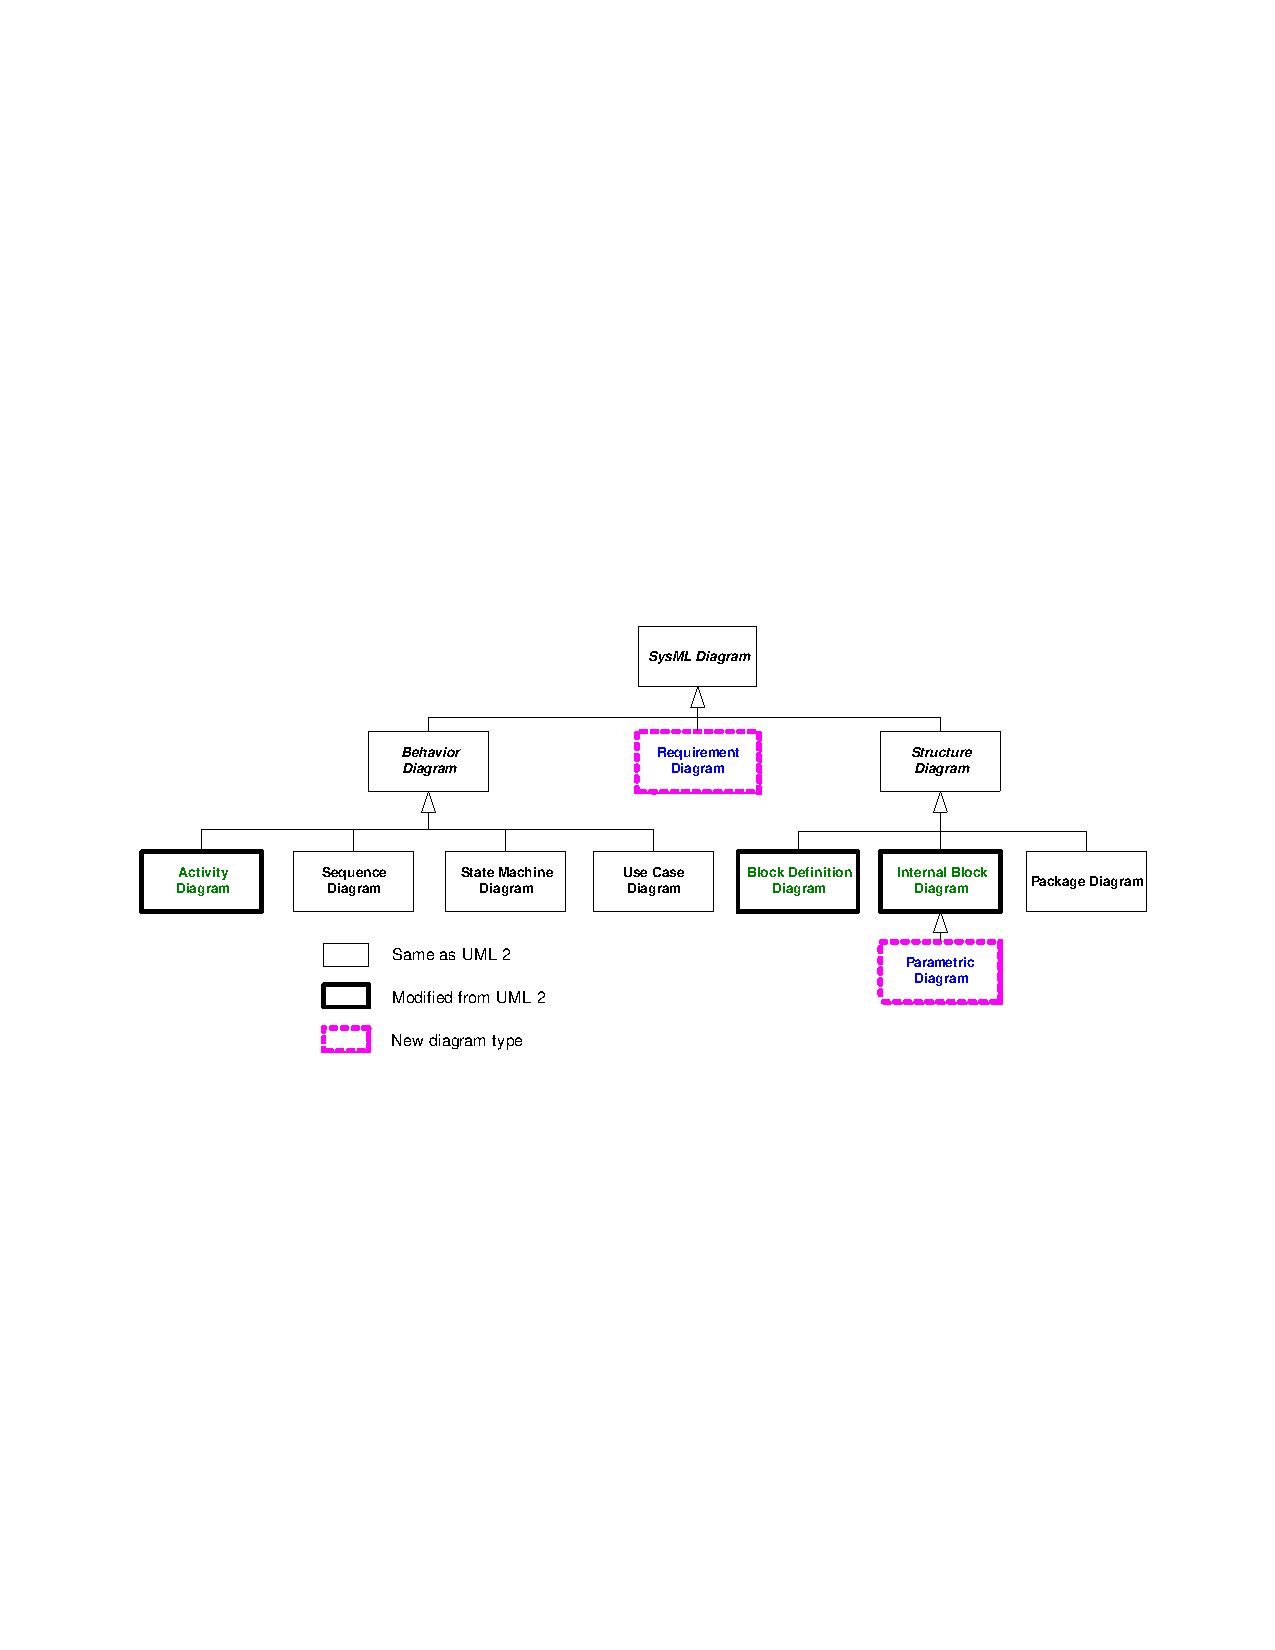
\includegraphics[scale=0.75]{figures/sysml_tax.pdf}
  \caption[SysML diagram taxonomy]{SysML diagram taxonomy \cite{sysmlspec}}
  \label{fig:sysmltax}
\end{figure}

The structure (static) diagrams can represent the system structures in varying degrees of transparency, for instance, Block Definition (black-box), Internal Block (white-box), or Requirement (declarative). The behavior (dynamic) diagrams represent the interactions of internal parts. For example, Activity Diagram describes the flow and the decisions of the component processes. Sequence Diagram extends the precision further by describing the sequence of the processes and what data they propagate in each step. 

The various diagram types in SysML enable the inclusion of system descriptions on different abstraction levels, so throughout all stages of the developmental cycle, the stakeholders---likely from various disciplines---can understand relevant diagrams without much efforts. However, one aspect SysML does not concentrate on is the ability to coordinate with external toolsets, especially if they do not adhere to the modeling language syntax in the first place. One who wishes to establish a ``live link" to SysML modelling environment from the outside will often find themselves working considerably on a conversion layer. Due to this reason, we incline not to consider it in the framework selection of this project.

SysML is a modelling language, not a framework per se. Yet there exists a number of platforms which utilize SysML to accomplish modelling and design activities, including the orchestration of models within the platform environment; one of them is IBM Rhapsody \cite{IBMSYSML}. This kind of platform inherits the previously mentioned disadvantages of SysML, i.e., cumbersome to incorporate external toolsets that do not adhere to the SysML syntax. However, we find the diagram approach in SysML keeps the execution workflow of the components very well organized. This is an attractive property for orchestration that we would like to have in our DT too.

\subsubsection{DevOps}
DevOps practice has received much attention, attributing to its emphasis on fast provisioning of business processes \cite{Ebert2016}. The core idea is that the development and operation are merged into one continuous loop of forward delivery and feedback (see Figure \ref{fig:devops}), often referred collectively as continuous integration and continuous deployment (CI/CD).

\begin{figure}[hbt!]
  \centering
  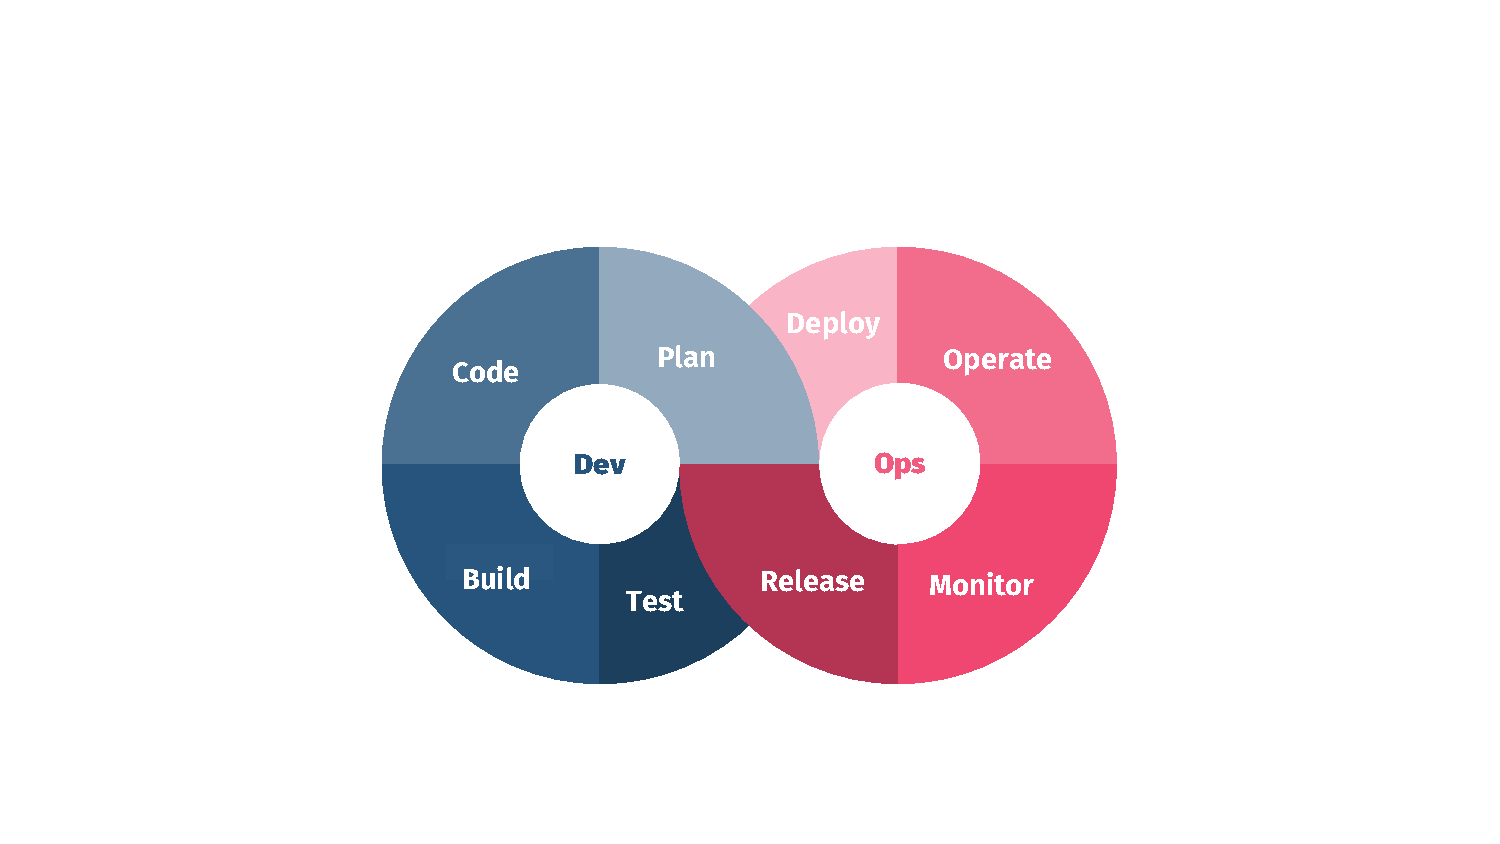
\includegraphics[scale=0.4]{figures/devops.pdf}
  \caption{DevOps concept portrayed by the infinite loop}
  \label{fig:devops}
\end{figure}

\begin{figure}[hbt!]
  \centering
  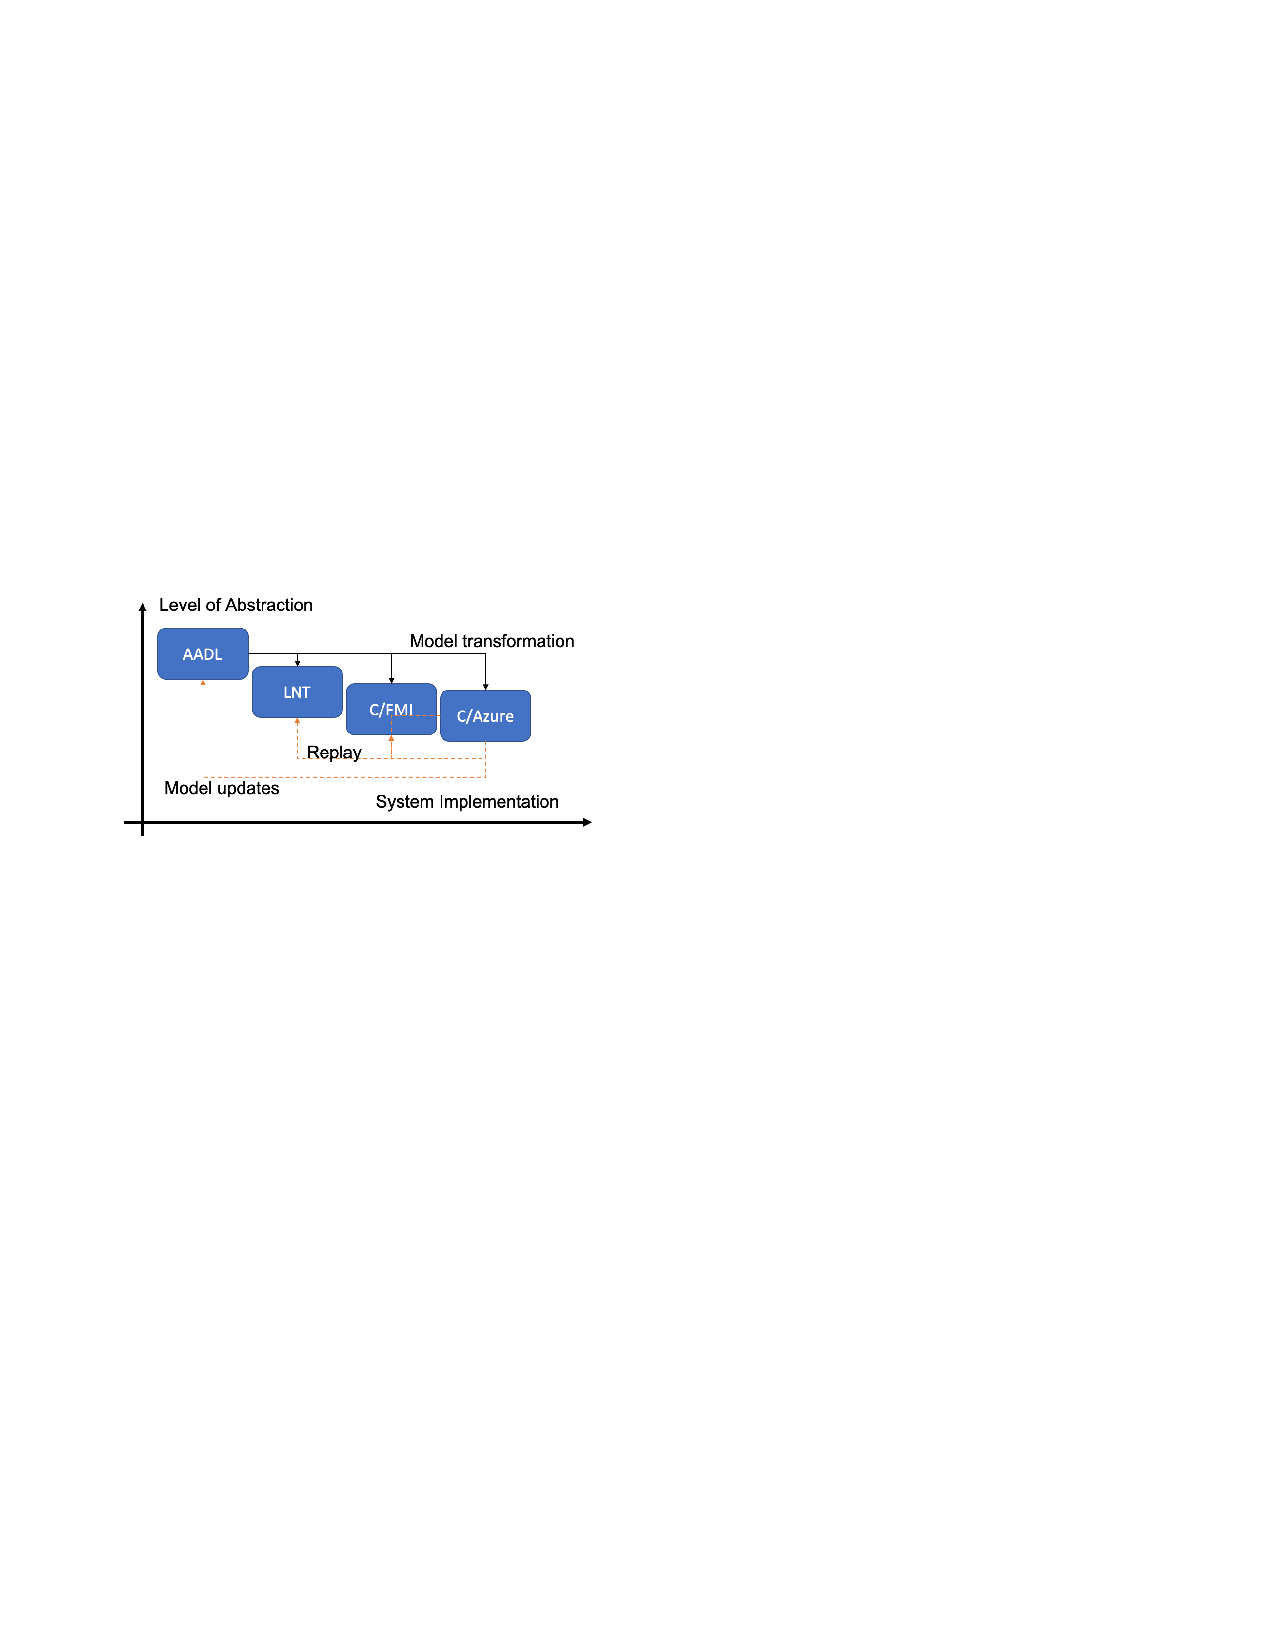
\includegraphics[scale=0.9]{figures/twinopsloop.pdf}
  \caption[TwinOps forward and feedback loop]{TwinOps forward and feedback loop \cite{Hugues2020}}
  \label{fig:twinopsloop}
\end{figure}

Hugues et al. \cite{Hugues2020} borrows this idea and proposes a DT variant of DevOps called TwinOps. In TwinOps, the ``Dev" part transcends to DT model integration and target code generation; and the ``Ops" part is overloaded with data collection and analysis in DTs. As illustrated in Figure \ref{fig:twinopsloop}, the black arrows are the code generation forwarded to various targets, and the orange arrows represent the data analytic feedback. In the work of Hugues, the exemplified case study of a building monitoring system utilizes the technology stack consisting of AADL, LNT, C, FMI, and Azure to build a pipeline. The AADL toolchain is responsible for specifying the modeling architecture as well as requirements. The LNT target enables model-checking. The C/FMI target supports modeling and simulation of the virtual entity. Finally the C/Azure target leverages a containerized cloud system to deploy execution command on the physical entity.

It is worth to note that under the DevOps presumption, the orchestration is implicit in TwinOps. The orchestration is embedded in the CI/CD pipeline for which the user takes the responsibility to configure the steps for transporting and transforming the model states.

TwinOps will be taken as a framework to be investigated further in Chapter \ref{ch:methodology}.

\subsubsection{SOA} 
As cloud services continue to gain popularity, there is a number of studies \cite{Preuveneers2018, Borghesi2021, Hung2022} that look into constructing DTs in line with SOA. In this approach, it regards either the VE models or the services in DTs as independent microservices. The VEs are often deployed as containers, and orchestrated by off-the-shelf applications such as Kubernetes \cite{Kubernetes}, for example, Kubernetes could use DNS for service discovery and exploits network traffic controls for scaling. This view of DTs provides the benefits of rapid deployment, as well as auto monitoring, scaling, and load balancing among other features which are found in commercial cloud services. 

As the number of entities introduced to the existing microservices pool continues growing, we can establish a machine-to-machine (M2M) network. An M2M network is characterized by localized---in the sense of not requiring a powerful computing node from another distant network---exchanges of data and services among the entities. It is contrary to the old-fashioned approach where only one central mainframe responsible for all services. This feature is considered attractive under the DT orchestration context, since DT models are also logically separated; can exchange data and contribute to the services. 

SOA will be the basis of the ThingsBoard framework which we choose to investigate further in this project. More will be discussed in Chapter \ref{ch:methodology}.

\subsubsection{Actor-orientated model}
An actor-orientated model as used by the Ptolemy II framework coordinates actors in various models of computation (MoC) while maintaining strong semantics of each individual model \cite{Ptolemaeus2014}. The term ``actor" refers to a self-contained component in the system that can interface with other components, comparable to the ``object" in object-oriented programming (OOP). The main difference is while OOP objects interface through ``methods", the actors interface primarily through ``ports". The notion of MoC refers to an abstract collection of rules that govern the interaction between components in a design. It is analogous to the ``laws of physic" that are used to describe a given system. Figure \ref{fig:moc} shows\footnote{In the figure, the meanings of the colors were never specified in the original source} a summary of the relationship between MoCs, which are represented as ``domains" in Ptolemy II.

\begin{figure}[htb!]
  \centering
  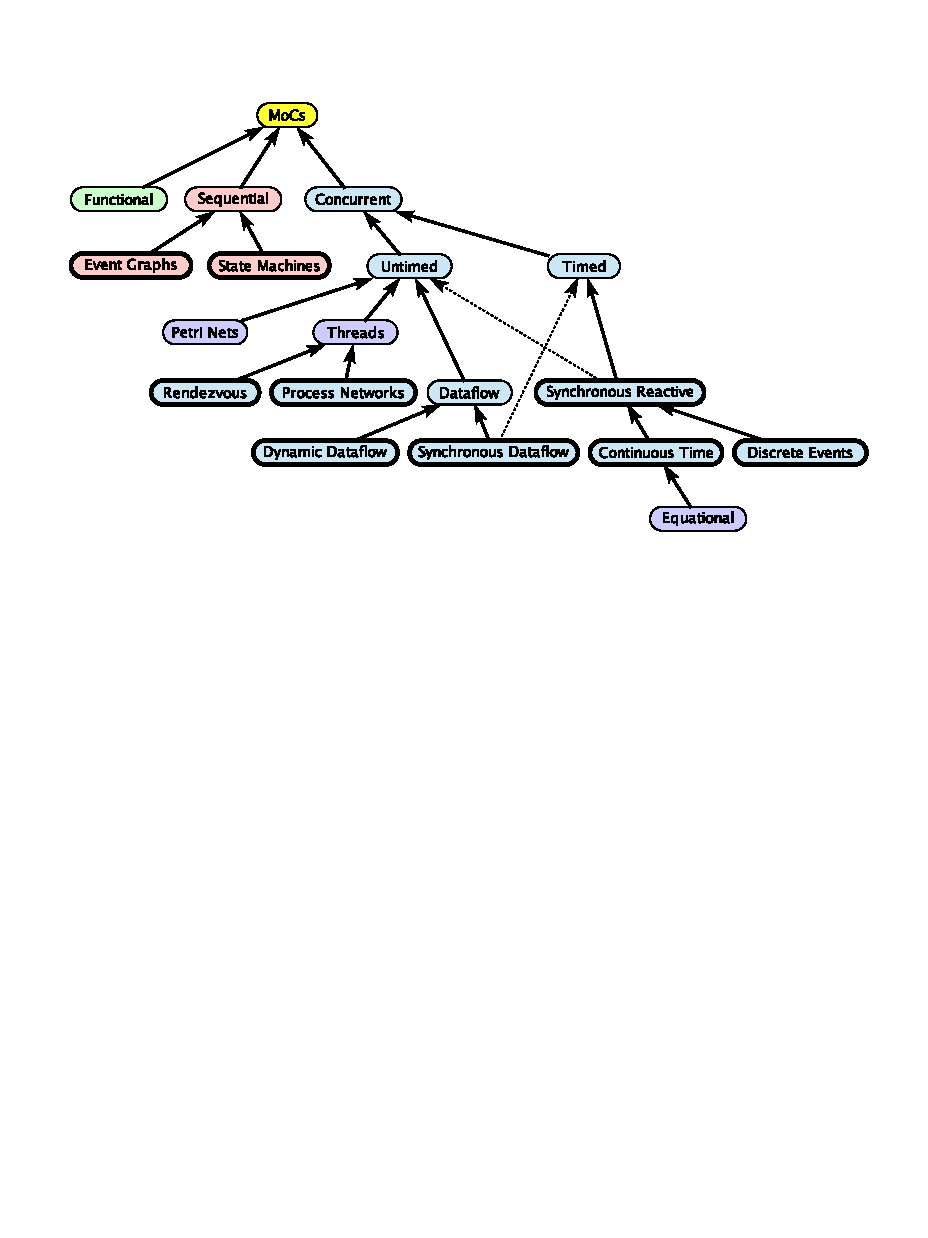
\includegraphics[scale=0.8]{figures/moc.pdf}
  \caption[MoCs relationship]{MoCs relationship \cite{Ptolemaeus2014}. The nodes with thick edges are currently supported by the latest Ptolemy II version. Bold arrows indicate primary associations. Dotted arrows denote alternative associations with either timed or untimed mode.}
  \label{fig:moc}
\end{figure}

We will consider Ptolemy II as one of the frameworks to be investigated further in Chapter \ref{ch:methodology}. Below is a list of some MoCs that we consider more applicable to the DT contexts of manufacturing and production plant:

\begin{itemize}

  \item Process network (PN) \cite{Tripakis2014} : scheduling for concurrent distributed processes. It has a benefit of determinacy as long as there is a unique solution to the balance equations of the nodes within the network. 

  \item Finite state machine (FSM): captures control-dominated behaviors. 
  
  \item Discrete event (DE): suited for modelling the behaviors of complex systems over time, e.g., queuing systems.
  
  \item Continuous time: essential for solving ODEs.

\end{itemize}

\subsection{DT in bioprocessing} \label{sec:dtbio}
In this subsection a number of case studies will be reviewed. They all share the common theme of bioprocess production, which is also shared by the microbrewery DT in our case. We will briefly discuss the integration and orchestration techniques used by these studies.

A study of enzyme production \cite{Mears2017} proposes a model-based strategy to maximize the final fill of a fed-batch process. The study demonstrates a multi-layer approach for orchestration. The cascaded layers are separated by a supervisory layer and a regulatory layer. The supervisory layer implements a mechanistic model that calculates the required start fill. This is the model-based batch planning for initial conditions. The model's parameters are re-fitted using a least squares approach. As for the regulatory layer, the calculated feed rate is adjusted by a PID controller. The results show that orchestrating an additional layer makes the final yield more predictable, which in turn makes the downstream resource allocation easier to manage.

Lopez et al. \cite{Lopez2020} propose a DT of ethanol fermentation. The researchers use a data-driven soft sensor that takes the online spectroscopy measurements to compute the glucose  concentration---referred as process variable (PV)---in real-time. PV is then used as the input to a PID algorithm in order to generate a final control signal---referred as manipulated variable (MV)--- that adjusts the feed rate of the controlled pump. The PV-MV transformation in this example showcases how monitoring models and controlling models can be integrated.

In their manufacturing platform for antibodies, Feidl et al. \cite{Feidl2020} manage to build a process‐wide control with a SCADA system. The system collects unit-relevant data streams from each process unit, then converts to a centralized data storage, which contextualizes and adds a timestamp to each data point, in which the data is transformed to process-relevant. Afterward, the SCADA system is able to send newly determined setpoints to the respective local control units. Hence, an automated end‐to‐end integration of the supervisory control with the data acquisition system is achieved. 

Eppinger and colleagues from Siemens \cite{Eppinger2021} design a DT for ketchup production. The control objectives are evaluated by a set of Key Performance Indicators (KPI). The DT firstly obtains the model parameters from historical data through a machine learning based analysis. A hybrid model that combines an equation-driven model and a data-driven model is then developed before being applied a model order reduction process, such that it can be made compatible with the real-time hard sensors. Once the reduced model is generated, the soft sensors---referred as virtual sensors---can be synthesized and be used to predict the KPIs. Finally, given all available information, the agent of the reinforcement learning algorithm executes actions toward the physical plant and tunes itself with respect to target KPIs by using feedbacks. This study explains a method to orchestrate hybrid models under time critical constraints. 

\section{Summary}
In Section \ref{sec:sota} we surveyed the recent development of DTs regarding monitoring, modelling, and controlling. They are not directly within the topics of integration and orchestration, but the information will be helpful in choosing technologies for our DT building blocks. Besides, some properties of integration and orchestration in fact arise under the influences of these aspects, as they are arguably the backbone of all DT services.

In Section \ref{sec:relatedwork}, we described the approaches for integration, the approaches for orchestration, and multiple DT case studies in the bioprocessing domain, in that order. For integration standards, we presented CAPE-OPEN and FMI, the former targets bio-chemistry applications, while the latter is more general. For orchestration strategies, we reviewed four distinctive styles but decided only three are suitable for our DT. The SysML approach, despite its excellence at propagating system-level descriptions, lacks the features for collaborating with external toolsets. 

